\documentclass [a4paper]{article}
\usepackage{graphicx, amsmath,amsfonts}
\usepackage[a4paper, total={8.5in, 13in}, margin=1in]{geometry}
\bibliographystyle{plain}
\usepackage{listings}
\usepackage{xcolor}
\lstset{
    language=Python,
    basicstyle=\ttfamily\small,
    keywordstyle=\color{blue},
    commentstyle=\color{gray},
    stringstyle=\color{red},
    showstringspaces=false,
    frame=single,
    breaklines=true,
    numbers=left,
    numberstyle=\tiny\color{gray},
    tabsize=4,
}

\title{MAT 196 Laboratory Exercise No.3}
\author{Jeanne Marie B. Quiñanola}
\date{\today}

\begin{document}

\maketitle

\section{Introduction}
In difference equations, the changes in states of a system are modeled over discrete intervals. In most cases, the discrete intervals represent time intervals, and therefore the letter \(t\) is used to denote the time variable.
A form of the difference equation that will be encountered most often is 
\[
x_{t + k} + a_1 x_{t+k-1} + \ldots + a_{k-1} x_{t+1} + a_k x_t = b_t, \quad t = 0, 1,\ldots\]

The order of the difference equation is \(k\), provided \(a_k \neq 0\). The coefficients are assumed to be real and the functions are real-valued. The coefficients \(a_j\), \(j = 1, \ldots, k\), can be functions of \(t\) and state variables \(x_i\) for \(i = t, \ldots, t + k - 1\). The function \(b_t\) on the right-hand side of the equation may depend on \(t\) but not on the state variables.

If the coefficients \(a_j\), \(j = 1, \ldots, k\) in the equation are constant or depend on \(t\) but do not depend on the state variables, then the difference equation is said to be linear. Otherwise, it is said to be nonlinear. In addition, if the difference equation is linear and \(b_t = 0\) for all \(t\), then it is said to be homogeneous; otherwise, it is said to be nonhomogeneous.

Now, a higher-order linear difference equation can be converted to a first-order linear system. Thus, a higher-order linear difference equation can be considered a special case of a first-order linear difference system. Consider the \(k\)th-order linear difference equation
\[
x(t + k) + a_1 x(t + k - 1) + \dots + a_{k-1} x(t + 1) + a_k x(t) = b(t),
\]
where for convenience \(x_t\) is denoted as \(x(t)\), \(b_t\) as \(b(t)\), and so on. To transform this \(k\)th-order equation to a first-order system, we define the following vector of states.

Let \(Y(t)\) be a \(k\)-dimensional vector,
\[
Y(t) = {\begin{pmatrix} y_1(t) \\ y_2(t) \\ \vdots \\ y_k(t) \end{pmatrix}}^T,
\]
satisfying the following:
\[
y_1(t) = x(t),
\]
\[
y_2(t) = x(t + 1),
\]
\[
\vdots
\]
\[
y_{k-1}(t) = x(t + k - 2),
\]
\[
y_k(t) = x(t + k - 1).
\]
The first element \(y_1(t)\) is the solution \(x(t)\). Next, a first-order difference equation in \(y\) is formed,
\[
y_1(t + 1) = y_2(t),
\]
\[
y_2(t + 1) = y_3(t),
\]
\[
\vdots
\]
\[
y_{k-1}(t + 1) = y_k(t),
\]
\[
y_k(t + 1) = -a_1 y_{k}(t) - \dots - a_{k-1} y_2(t) - a_k y_1(t) + b(t).
\]
The last equation is obtained from the difference equation above. The first-order system can be written in matrix form,
\[
Y(t + 1) = A Y(t) + B.
\]
where
\[
A = \begin{pmatrix}
0 & 1 & 0 & \dots & 0 \\
0 & 0 & 1 & \dots & 0 \\
\vdots & \vdots & \vdots & \ddots & \vdots \\
0 & 0 & 0 & \dots & 1 \\
-a_k & -a_{k-1} & -a_{k-2} & \dots & -a_1 \\
\end{pmatrix}
\quad \text{and} \quad
B = \begin{pmatrix}
0 \\
0 \\
\vdots \\
0 \\
b(t) \\
\end{pmatrix}.
\]
Consider the homogeneous system \( X(t+1) = AX(t) \), where \( X(t) = (x_1(t), x_2(t), \ldots, x_k(t))^T \) and \( A = (a_{ij}) \) is a \( k \times k \) constant matrix. This system has \( k \) linearly independent solutions, denoted by \( \{X_i(t)\}_{i=1}^k \), similar to the case of a \( k \)-th order homogeneous scalar equation. The general solution can be expressed as:
\[
X(t) = \sum_{i=1}^k c_i X_i(t),
\]
where \( c_i \) are constants determined by initial conditions.
Now, let \( X(t+1) = AX(t) \), where \( A = (a_{ij}) \) is a \( k \times k \) constant matrix. Assume that \( X(t) = \lambda^t V \), where \( V \) is a nonzero \( k \)-column vector and \( \lambda \) is a constant. Substituting \( \lambda^t V \) into the linear system yields:
\[
\lambda^{t+1} V = A(\lambda^t V),
\]
which simplifies to:
\[
(A - \lambda I)V = 0,
\]
where \( I \) is the identity matrix and \( 0 \) is the zero vector. 

From linear algebra, we know that if \( \det(A - \lambda I) \neq 0 \), then the equation \( (A - \lambda I)V = 0 \) has a unique solution, which is the trivial solution \( V = 0 \). Nonzero solutions \( V \) are obtained if and only if the matrix \( A - \lambda I \) is singular, that is, if:
\[
\det(A - \lambda I) = 0.
\]
The following are the different cases of eigenvalues depending on the linear system given.\\

\textbf{Case 1:} Suppose the eigenvalues are real and the solutions, $i = 1, 2, \dots, k$, are linearly independent. Then the general solution to the linear system $X(t + 1) = AX(t)$ can be expressed as
\[
X(t) = \sum_{i=1}^k c_i \lambda_i^t V_i. 
\]
(Note that the eigenvectors are also real-valued because $A$ has real entries.)

\textbf{Case 2:} Suppose matrix $A$ has $k$ distinct eigenvalues. Then it follows that there are $k$ linearly independent eigenvectors (Ortega, 1987), and the solution can still be written as in (1.19). The entries $\lambda_i^t V_i$ may not have real values.

\textbf{Case 3:} In the other cases, when the eigenvalues are complex or the eigenvectors are not independent, the general solution includes such terms as $t^n \lambda_i^t V_i$ or $t^n \lambda_i^t \cos(c_i t) V_i$.\cite{linda}
\newpage

With that said, the following problem deals with the number of red blood cells (RBCs) circulating in the blood. Here we will present it as a discrete problem to be modeled by difference equations.

In the circulatory system, the red blood cells (RBCs) are constantly being destroyed and replaced. Since these cells carry oxygen throughout the body, their number must be maintained at some fixed level. The spleen filters out and destroys a fraction of the cells daily and the bone marrow produces a number proportional to the number lost on the previous day. \cite{edelstein2005mathematical}

The cell count on day \(t\) is modeled as follows\\

\begin{align*}
\begin{cases}
  R(t+1) &= (1 - f)R(t) + M(t), \\
  M(t+1) &= \gamma f R(t).
\end{cases}    
\end{align*}

where: 
\begin{align*}
  R(t) & = \text{number of RBCs in circulation on day } t, \\
  M(t) & = \text{number of RBCs produced by marrow on day } t, \\
  f & = \text{fraction of RBCs removed by spleen}, 0< f<1,\\
  \gamma & = \text{production constant}   \quad (\gamma > 0) 
\end{align*}

In this paper, will convert the following system of equations into matrix form and determine its eigenvalues along with their corresponding eigenvectors. Additionally, we will analyze the behavior of the solutions \( R(t) \) and \( M(t) \) as \( t \) approaches infinity by examining the solutions for each cases.

\section{Analysis and Discussion}

Given the system of equations:
\[
\begin{cases}
R(t+1) = (1 - f) R(t) + M(t) \\
M(t+1) = \gamma f R(t)
\end{cases}
\]Let:
   \[
   X(t) = \begin{bmatrix} R(t) \\ M(t) \end{bmatrix}.
   \]Then the system can be rewritten in matrix form as:
   \[
   X(t+1) = A X(t)
   \]
where \( A \) is the matrix:
   \[
   A = \begin{bmatrix} 1 - f & 1 \\ \gamma f & 0 \end{bmatrix}.
   \]

To find the eigenvalues of \( A \), we solve the characteristic polynomial \(\det(A - \lambda I) = 0\), where \(\lambda\) is an eigenvalue and \(I\) is the identity matrix.

   The characteristic polynomial is:
   \[
   \det \begin{bmatrix} 1 - f - \lambda & 1 \\ \gamma f & -\lambda \end{bmatrix} = 0
   \]

   Expanding this determinant, we get:
   \[
   (1 - f - \lambda)(-\lambda) - (1)(\gamma f) = 0
   \]
   \[
   \lambda^2 - (1 - f)\lambda - \gamma f = 0
   \]

   Solving for \(\lambda\) we have: \\
   \[
   \lambda = \frac{(1 - f) \pm \sqrt{(1 - f)^2 + 4 \gamma f}}{2}
   \]

To examine how the solutions of \( R(t) \) and \( M(t) \) vary with different parameters, we will consider the following values of \( \gamma \) and \( f \).
   \begin{itemize}
       \item \( f = \frac{1}{2} \) and \( \gamma = \frac{1}{2} \)
       \item \( f = \frac{1}{2} \) and \( \gamma = 1 \)
       \item \( f = \frac{1}{2}\) and \( \gamma = \frac{3}{2} \)
   \end{itemize}
\subsection*{Case 1: \( f = \frac{1}{2} \) and \( \gamma = \frac{1}{2} \)}

\begin{align*}
   \lambda &= \frac{\left(1 - \frac{1}{2}\right) \pm \sqrt{\left(1 - \frac{1}{2}\right)^2 + 4 \left(\frac{1}{2}\right) \left(\frac{1}{2}\right)}}{2} \\
   &= \frac{\frac{1}{2} \pm \sqrt{\frac{1}{4} + 1}}{2} \\
   &= \frac{\frac{1}{2} \pm \sqrt{\frac{5}{4}}}{2} \\
   &= \frac{\frac{1}{2} \pm \frac{\sqrt{5}}{2}}{2} \\
   &= \frac{1 \pm \sqrt{5}}{4}.
\end{align*}

Hence, we have: 
   \[
   \lambda_1 = \frac{1 + \sqrt{5}}{4}, \quad \lambda_2 = \frac{1 - \sqrt{5}}{4}.
   \]

For \(f = \frac{1}{2}\) and \(\gamma = \frac{1}{2}\), we have: 

\[
     \begin{pmatrix} 1 - \frac{1}{2} - \lambda & 1 \\ \left(\frac{1}{2}\right) \left(\frac{1}{2}\right) & -\lambda \end{pmatrix}\mathbf{V} = 0
\]
\[
\begin{pmatrix} \frac{1}{2} - \lambda & 1 \\ \frac{1}{4} & -\lambda \end{pmatrix} \mathbf{V} = \mathbf{0}
\]


Substituting \(\lambda_1 = \frac{1 + \sqrt{5}}{4}\) we have:
\[
\begin{pmatrix} \frac{1 - \sqrt{5}}{4} & 1 \\ \frac{1}{4} & -\frac{1 + \sqrt{5}}{4} \end{pmatrix} \begin{pmatrix} v_1 \\ v_2 \end{pmatrix} = \textbf{0}
\]

This leads to the system of equations:
\begin{align*}
\begin{cases}
\frac{1 - \sqrt{5}}{4} v_1 + v_2 = 0 & \implies v_2 = -\frac{1 - \sqrt{5}}{4} v_1 \\[1em]
\frac{1}{4} v_1 - \frac{1 + \sqrt{5}}{4} v_2 = 0 &
\end{cases}
\end{align*}

Solving for \(v_1\) and \(v_2\) we have: 
\[
\frac{1}{4} v_1 + \frac{(1 + \sqrt{5})(1 - \sqrt{5})}{16}v_1  = 0
\]
\[
\frac{1}{4} v_1 - \frac{1}{4} v_1 = 0
\]
\[0=0\]

Any \(v_1 \in \mathbb{R}\) satisfies the equation.  Let \(v_1 = -4\).
Then, \(
v_2 = 1 - \sqrt{5}. 
\)

Thus, we have: 

\[
\begin{pmatrix} v_1 \\ v_2 \end{pmatrix} = \begin{pmatrix} -4 \\ 1 - \sqrt{5}\end{pmatrix}.
\]

Substituting \(\lambda_2 = \frac{1 - \sqrt{5}}{4}\) we have:
\[
\begin{pmatrix} \frac{1 + \sqrt{5}}{4} & 1 \\ \frac{1}{4} & -\frac{1 - \sqrt{5}}{4} \end{pmatrix} \begin{pmatrix} v_3 \\ v_4 \end{pmatrix} = \textbf{0}
\]

This leads to the system of equations:
\begin{align*}
\begin{cases}
\frac{1 + \sqrt{5}}{4} v_3 + v_4 = 0 & \implies v_4 = -\frac{1 + \sqrt{5}}{4} v_3 \\[1em]
\frac{1}{4} v_3 - \frac{1 - \sqrt{5}}{4} v_4 = 0 &
\end{cases}
\end{align*}

Solving for \(v_3\) and \(v_4\) we have: 
\[
\frac{1}{4} v_3 + \frac{(1 - \sqrt{5})(1 + \sqrt{5})}{16}v_3  = 0
\]
\[
\frac{1}{4} v_3 - \frac{1}{4} v_3 = 0
\]
\[0=0\]

Any \(v_3 \in \mathbb{R}\) satisfies the equation. Let \(v_3 = -4\).
Then,\(
v_4 = 1 + \sqrt{5} 
\).

Thus, we have: 

\[
\begin{pmatrix} v_3 \\ v_4 \end{pmatrix} = \begin{pmatrix} -4 \\ 1 + \sqrt{5}\end{pmatrix}.
\]

Hence, 
\[ X(t) = c_1{\left(\frac{1 + \sqrt{5}}{4}\right)}^t\begin{pmatrix}
    -4 \\ 1-\sqrt{5}
\end{pmatrix} + c_2{\left(\frac{1 - \sqrt{5}}{4}\right)}^t\begin{pmatrix}
    -4 \\ 1 +\sqrt{5}
\end{pmatrix} \quad c_1,c_2 \in \mathbb{R}.\]

\subsection*{Case 2: \( f = \frac{1}{2} \) and \( \gamma = 1 \)}

\begin{align*}
   \lambda &= \frac{\left(1 - \frac{1}{2}\right) \pm \sqrt{\left(1 - \frac{1}{2}\right)^2 + 4 \left(1\right) \left(\frac{1}{2}\right)}}{2} \\
   &= \frac{\frac{1}{2} \pm \sqrt{\frac{1}{4} + 2}}{2} \\
   &= \frac{\frac{1}{2} \pm \sqrt{\frac{9}{4}}}{2} \\
   &= \frac{\frac{1}{2} \pm \frac{3}{2}}{2} \\
   &= \frac{1 \pm 3}{4}.
\end{align*}

Thus, we have: 
\[
   \lambda_1 = 1, \quad \lambda_2 = -\frac{1}{2}.
\]

For \(f = \frac{1}{2}\) and \(\gamma = 1\), we have: 

\[
     \begin{pmatrix} 1 - \frac{1}{2} - \lambda & 1 \\ \left(\frac{1}{2}\right) \left(1\right) & -\lambda \end{pmatrix}\mathbf{V} = 0
\]

\[
\begin{pmatrix} \frac{1}{2} - \lambda & 1 \\ \frac{1}{2} & -\lambda \end{pmatrix} \mathbf{V} = \mathbf{0}
\]

Substituting \(\lambda_1 = 1\) we have:
\[
\begin{pmatrix} -\frac{1}{2}  &  1 \\ \frac{1}{2} & -1 \end{pmatrix} \begin{pmatrix} v_1 \\ v_2 \end{pmatrix} = \mathbf{0}
\]

This leads to the system of equations:
\begin{align*}
\begin{cases}
-\frac{1}{2} v_1 + v_2 = 0 & \implies v_2 = \frac{1}{2} v_1 \\[1em]
\frac{1}{2} v_1 - v_2 = 0 &
\end{cases}
\end{align*}

Let \(v_1 = 2\).
Then \(v_2 = 1.\)

Thus, we have: 

\[
\begin{pmatrix} v_1 \\ v_2 \end{pmatrix} = \begin{pmatrix} 2 \\ 1 \end{pmatrix}.
\]

Substituting \(\lambda_2 = -\frac{1}{2}\) we have:
\[
\begin{pmatrix} 1  &  1 \\ \frac{1}{2} & \frac{1}{2} \end{pmatrix} \begin{pmatrix} v_3 \\ v_4 \end{pmatrix} = \mathbf{0}
\]

This leads to the system of equations:
\begin{align*}
\begin{cases}
v_3 + v_4 = 0 & \implies v_3 = -v_4 \\[1em]
\frac{1}{2}v_3 + \frac{1}{2} v_4 = 0 &
\end{cases}
\end{align*}

Let \(v_4 = 1\).
Then \(v_3 = -1.\)

Thus, we have: 

\[
\begin{pmatrix} v_3 \\ v_4 \end{pmatrix} = \begin{pmatrix} -1 \\ 1 \end{pmatrix}.
\]

Hence, 
\[ X(t) = c_1\begin{pmatrix}
    2 \\ 1
\end{pmatrix} + c_2{\left(-\frac{1}{2}\right)}^t\begin{pmatrix}
    -1\\ 1 
\end{pmatrix} \quad c_1,c_2 \in \mathbb{R}.\]

\subsection*{Case 3: \( f = \frac{1}{2} \) and \( \gamma = \frac{3}{2} \)}

\begin{align*}
   \lambda &= \frac{\left(1 - \frac{1}{2}\right) \pm \sqrt{\left(1 - \frac{1}{2}\right)^2 + 4 \left(\frac{3}{2}\right) \left(\frac{1}{2}\right)}}{2} \\
   &= \frac{\frac{1}{2} \pm \sqrt{\frac{1}{4} + 3}}{2} \\
   &= \frac{\frac{1}{2} \pm \sqrt{\frac{13}{4}}}{2} \\
   &= \frac{\frac{1}{2} \pm \frac{\sqrt{13}}{2}}{2} \\
   &= \frac{1 \pm \sqrt{13}}{4}.
\end{align*}

Hence, we have: 
   \[
   \lambda_1 = \frac{1 + \sqrt{13}}{4}, \quad \lambda_2 = \frac{1 - \sqrt{13}}{4}.
   \]

For \(f = \frac{1}{2}\) and \(\gamma = \frac{1}{2}\), we have: 

\[
     \begin{pmatrix} 1 - \frac{1}{2} - \lambda & 1 \\ \left(\frac{3}{2}\right) \left(\frac{1}{2}\right) & -\lambda \end{pmatrix}\mathbf{V} = 0
\]
\[
\begin{pmatrix} \frac{1}{2} - \lambda & 1 \\ \frac{3}{4} & -\lambda \end{pmatrix} \mathbf{V} = \mathbf{0}
\]


Substituting \(\lambda_1 = \frac{1 + \sqrt{13}}{4}\) we have:
\[
\begin{pmatrix} \frac{1 - \sqrt{13}}{4} & 1 \\ \frac{3}{4} & -\frac{1 + \sqrt{13}}{4} \end{pmatrix} \begin{pmatrix} v_1 \\ v_2 \end{pmatrix} = \textbf{0}
\]

This leads to the system of equations:
\begin{align*}
\begin{cases}
\frac{1 - \sqrt{13}}{4} v_1 + v_2 = 0 & \implies v_2 = -\frac{1 - \sqrt{13}}{4} v_1 \\[1em]
\frac{3}{4} v_1 - \frac{1 + \sqrt{13}}{4} v_2 = 0 &
\end{cases}
\end{align*}
\newpage
Solving for \(v_1\) and \(v_2\) we have: 
\[
\frac{3}{4} v_1 + \frac{(1 + \sqrt{13})(1 - \sqrt{13})}{16}v_1  = 0
\]
\[
\frac{3}{4} v_1 - \frac{3}{4} v_1 = 0.
\]
\[0=0\]

Any \(v_1 \in \mathbb{R}\) satisfies the equation. Let \(v_1 = -4\).
Then, \(
v_2 = 1 - \sqrt{13}. 
\)

Thus, we have: 

\[
\begin{pmatrix} v_1 \\ v_2 \end{pmatrix} = \begin{pmatrix} -4 \\ 1 - \sqrt{13}\end{pmatrix}.
\]

Substituting \(\lambda_2 = \frac{1 - \sqrt{13}}{4}\) we have:
\[
\begin{pmatrix} \frac{1 + \sqrt{13}}{4} & 1 \\ \frac{3}{4} & -\frac{1 - \sqrt{13}}{4} \end{pmatrix} \begin{pmatrix} v_3 \\ v_4 \end{pmatrix} = \textbf{0}
\]

This leads to the system of equations:
\begin{align*}
\begin{cases}
\frac{1 + \sqrt{13}}{4} v_3 + v_4 = 0 & \implies v_4 = -\frac{1 + \sqrt{13}}{4} v_3 \\[1em]
\frac{3}{4} v_3 - \frac{1 - \sqrt{13}}{4} v_4 = 0 &
\end{cases}
\end{align*}

Solving for \(v_3\) and \(v_4\) we have: 
\[
\frac{3}{4} v_3 + \frac{(1 - \sqrt{13})(1 + \sqrt{13})}{16}v_3  = 0
\]
\[
\frac{3}{4} v_3 - \frac{3}{4} v_3 = 0
\]
\[0=0\]

Any \(v_3 \in \mathbb{R}\) satisfies the equation.Let \(v_3 = -4\).
Then,\(
v_4 = 1 + \sqrt{13} 
\).

Thus, we have: 

\[
\begin{pmatrix} v_3 \\ v_4 \end{pmatrix} = \begin{pmatrix} -4 \\ 1 + \sqrt{13}\end{pmatrix}.
\]

Hence, 
\[ X(t) = c_1{\left(\frac{1 + \sqrt{13}}{4}\right)}^t\begin{pmatrix}
    -4 \\ 1-\sqrt{13}
\end{pmatrix} + c_2{\left(\frac{1 - \sqrt{13}}{4}\right)}^t\begin{pmatrix}
    -4 \\ 1 +\sqrt{13}
\end{pmatrix} \quad c_1,c_2 \in \mathbb{R}.\]
\newpage

\section{Convergence Analysis}

\subsection*{Case 1: \( f = \frac{1}{2} \) and \( \gamma = \frac{1}{2} \)}

For the first solution 
\[
X(t) = c_1{\left(\frac{1 + \sqrt{5}}{4}\right)}^t\begin{pmatrix} -4 \\ 1-\sqrt{5} \end{pmatrix} + c_2{\left(\frac{1 - \sqrt{5}}{4}\right)}^t\begin{pmatrix} -4 \\ 1 +\sqrt{5} \end{pmatrix}, \quad c_1, c_2 \in \mathbb{R},
\]
we observe that both terms converge to zero as \( t \to \infty \). Specifically, 
\[
\left| \frac{1 + \sqrt{5}}{4} \right| \approx 0.809,
\]
which is less than 1, so 
\[
c_1{\left(\frac{1 + \sqrt{5}}{4}\right)}^t \to 0
\]
as \( t \to \infty \). 
Similarly, 
\[
\left| \frac{1 - \sqrt{5}}{4} \right| \approx 0.309,
\]
whose absolute value is also less than 1, so the term 
\[
c_2{\left(\frac{1 - \sqrt{5}}{4}\right)}^t \to 0
\]
as well. 
Thus, as \(t \to \infty\), both components of \(X(t)\) approach zero, and consequently, 
\[
X(t) \to 0
\]
regardless of the values of \(c_1\) and \(c_2\).

\subsection*{Case 2: \( f = \frac{1}{2} \) and \( \gamma = 1 \)}

In the second solution 

\[
X(t) = c_1\begin{pmatrix} 2 \\ 1 \end{pmatrix} + c_2{\left(-\frac{1}{2}\right)}^t\begin{pmatrix} -1\\ 1 \end{pmatrix}, \quad c_1, c_2 \in \mathbb{R},
\]
the first term \(c_1\begin{pmatrix} 2 \\ 1 \end{pmatrix}\) is a constant vector that remains unchanged as \(t\) varies. The second term, \(\left| -\frac{1}{2} \right| = \frac{1}{2}\), oscillates in sign and converges to zero as \(t \to \infty\). Consequently, as \(t\) approaches infinity, \(X(t)\) converges to 

\[
c_1\begin{pmatrix} 2 \\ 1 \end{pmatrix},
\]
indicating that the limit is determined entirely by the constant vector and \(c_1\).

\newpage
\subsection*{Case 3: \( f = \frac{1}{2} \) and \( \gamma = \frac{3}{2} \)}

For the third solution 

\[
X(t) = c_1{\left(\frac{1 + \sqrt{13}}{4}\right)}^t\begin{pmatrix}
    -4 \\ 1-\sqrt{13}
\end{pmatrix} + c_2{\left(\frac{1 - \sqrt{13}}{4}\right)}^t\begin{pmatrix}
    -4 \\ 1 +\sqrt{13}
\end{pmatrix} \quad (c_1,c_2 \in \mathbb{R}),
\]
we observe that, 
\[
\left| \frac{1 + \sqrt{13}}{4} \right| \approx 1.151,
\]
which is greater than 1, so 
\[
c_1{\left(\frac{1 + \sqrt{13}}{4}\right)}^t \to \infty
\]
as \( t \to \infty \). 
Meanwhile, 
\[
\left| \frac{1 - \sqrt{13}}{4} \right| \approx 0.651,
\]
whose absolute value is also less than 1, so the term 
\[
c_2{\left(\frac{1 - \sqrt{13}}{4}\right)}^t \to 0.
\]
Thus, as \(t \to \infty\), \(X(t)\) approaches \(\infty\), if  \(c_1  <  0\)  and \(-\infty\) if \(c_1 >0\).

\section{Numerical Simulations}

\begin{figure}[h] 
    \centering 
    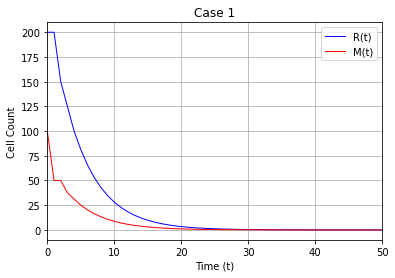
\includegraphics[width=0.80\textwidth]{Case 1.png} 
\end{figure}
\newpage
\begin{figure}[h]
    \centering 
    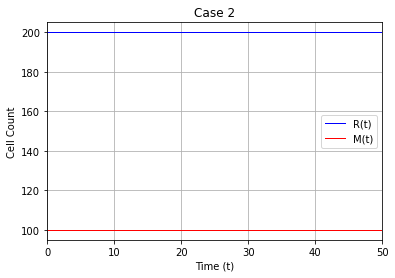
\includegraphics[width=0.80\textwidth]{Case 2.png} 
\end{figure}
\begin{figure}[h] 
    \centering 
    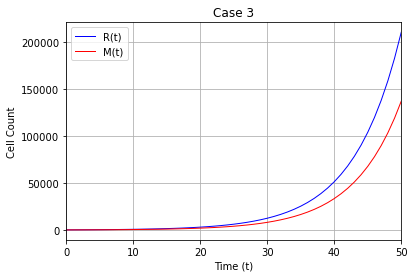
\includegraphics[width=0.80\textwidth]{Case 3.png} 
\end{figure}
\newpage

\section{Python Code for Cell Count Simulation}

Below is the Python code used for simulating cell counts over time:

\begin{lstlisting}[language=Python]
import numpy as np
from numpy import zeros
import matplotlib.pyplot as plt

# Time points
T = 50
index_set = range(T + 1)

# Initialize arrays for R and M
R = zeros(len(index_set))
M = zeros(len(index_set))

# Initial conditions
R[0] = 200
M[0] = 100

# Case 1
f = 0.5
gamma = 0.5

for t in index_set[0:T]:
    R[t + 1] = (1 - f) * R[t] + M[t]
    M[t + 1] = gamma * f * R[t]

# Plot results
plt.plot(index_set, R, 'b-', linewidth=1.0, label='R(t)')
plt.plot(index_set, M, 'r-', linewidth=1.0, label='M(t)')
plt.xlabel("Time (t)")
plt.ylabel("Cell Count")
plt.title("Case 1")
plt.legend(loc="best")
plt.xlim(0, 50)
plt.grid()
plt.show()

# Case 2
f = 0.5
gamma = 1.0

for t in index_set[0:T]: 
    R[t + 1] = (1 - f) * R[t] + M[t]
    M[t + 1] = gamma * f * R[t]

# Plot results
plt.plot(index_set, R, 'b-', linewidth=1.0, label='R(t)')
plt.plot(index_set, M, 'r-', linewidth=1.0, label='M(t)')
plt.xlabel("Time (t)")
plt.ylabel("Cell Count")
plt.title("Case 2")
plt.legend(loc="best")
plt.xlim(0, 50)
plt.grid()
plt.show()
\end{lstlisting}

\newpage  

\begin{lstlisting}[language=Python]
# Case 3
f = 0.5
gamma = 1.5

for t in index_set[0:T]:
    R[t + 1] = (1 - f) * R[t] + M[t]
    M[t + 1] = gamma * f * R[t]

# Plot results
plt.plot(index_set, R, 'b-', linewidth=1.0, label='R(t)')
plt.plot(index_set, M, 'r-', linewidth=1.0, label='M(t)')
plt.xlabel("Time (t)")
plt.ylabel("Cell Count")
plt.title("Case 3")
plt.legend(loc="best")
plt.xlim(0, 50)
plt.grid()
plt.show()
\end{lstlisting}


\section{Summary and Conclusions}
In this study, we analyzed a mathematical model representing the dynamics of red blood cell production and destruction within the circulatory system. By exploring various parameter configurations, we demonstrated the behavior of the system through both theoretical convergence analysis and numerical simulations.

The findings indicate that different values of the fraction of cells removed by the spleen (\(f\)) and the production constant (\(\gamma\)) significantly impact the stability and convergence of red blood cell counts over time. 

In the analysis of red blood cell dynamics over time, the solutions for \( R(t) \), the count of circulating red blood cells, and \( M(t) \), the count of red blood cells produced by the marrow, reveal distinct patterns depending on the values of \( f \) (the fraction of cells removed by the spleen) and \( \gamma \) (the production constant). 

Based on the convergence analysis and numerical simulations, we have the following. 

In case 1, where \( f = 0.5 \) and \( \gamma = 0.5 \), both \( R(t) \) and \( M(t) \) eventually converges to 0. This shows that given the said parameters, the number of red blood cells in circulation denoted by \(R(t)\) and the number of red blood cells produced by the marrow \(M(t)\) tend to decrease overtime. 

In case 2, with \( f = 0.5 \) and \( \gamma = 1.0 \), both \( R(t) \) and \( M(t) \) remains constant over time. This shows that given the said parameters, the number of red blood cells in circulation denoted by \(R(t)\) and the number of red blood cells produced by the marrow denoted by \(M(t)\) remains stable overtime. 

In case 3, for \( f = 0.5 \) and \( \gamma = 1.5 \), both \( R(t) \) and \( M(t) \) diverges to infinity.  This shows that given the said parameters, the number of red blood cells in circulation denoted by \(R(t)\) and the number of red blood cells produced by the marrow denoted by \(M(t)\) increases overtime. 

Overall, this paper highlights the intricate relationships within biological systems and the importance of mathematical modeling in understanding complex physiological processes.


\bibliography{citation} 
\end{document}
 